\chapter{Evaluation}\label{chap:evaluation}
This chapter describes the tests and experiments we setup in order to evaluate our solution. 
We setup \num{4} tests, one in each of the following sections. 
The first test, described in \Cref{sec:gestureperformance}, we perform is to measure the performance of the gesture recognizer described in \Cref{ref to Gesture Recognizer}. 
Then we evaluate the correctness of the gesture recognizer in \Cref{sec:gesturecorrectness}.
To test the precision of our indoor location, we perform precision tests on the Estimote SDK in \Cref{sec:estimoteprecision}.
Finally we test the system as a whole in \Cref{sec:systemcorrectness}.

\section{Performance of Gesture Recognition}\label{sec:gestureperformance}
Gesture recognition is a core part of our solution and it is being performed often. 
Since the gesture recognition is being performed by a device with somewhat low performance,
it is important that the gesture recognition is not computationally heavy.
In \Cref{sec:requirements-specification} we set a requirement of less than \SI{200}{\milli\second} for each gesture recognition.
We test the performance by gradually populating the database with gesture traces, 
and see how fast we can recognize a random gesture input.
We expect the number of gesture traces in the database to increase the recognition time.

For this setup, we add five gesture traces at a time. 
This is to simulate training a gesture five times, 
as recommended by the \$3 Gesture Recognition paper \cite{threedollar}. 
We then generate a random gesture input, 
and run the recognition function on it ten times, 
logging the execution time.
We repeat this until there is a total of \num{100} gesture traces in the database, 
which corresponds to \num{20} unique gestures.

We performed this test six times on an iPhone 5, 
with a \SI{1.3}{\giga\hertz} dual-core ARM processor and \SI{1}{\giga\byte} RAM, running iOS 9.1.
This device is more powerful than most wearables, 
but newer wearables such as the Samsung Gear S2 has a \SI{1}{\giga\hertz} dual core CPU with \SI{512}{\mega\byte} RAM, 
so the results from this section are comparable with newer and upcoming wearable devices.

\begin{figure}[!htb]
    \centering
    \begin{tikzpicture}
  \begin{axis}[ybar,bar width=2pt]
    \addplot table[x=gestureNo, y=time] {data/three-dollar-test-results/results/10xrecognize/2015-11-25 12.36.29.csv};   
  \end{axis}
\end{tikzpicture}
    \caption{Graph showing the time of recognizing gestures, with increasing number of gesture traces. Each unique gesture is training \num{5} times.}
    \label{fig:performancegraph}
\end{figure}

During testing we noticed that the ``Three Dollar Gesture Recognizer'' used a high amount of memory. 
Furthermore it did not properly release this memory, 
and as a result the application would terminate during tests, 
if we ran them for too long.
\Cref{fig:threedollarmemory} shows the amount of memory, 
used by our application, 
in a timespan of one minute and thirteen seconds, 
starting at the point where the application was launched on the iPhone. 
The first dotted line shows the time when the test began, 
and the second dotted line shows when the test finished, 
and where the \$3 Gesture Recognizer started cleaning up its resources.
However, as the graph shows, the memory use stays high after cleanup. %Thalley: Kunne det ikke blot være pga. iOS's måde at håndtere memory på? 
This issue is the reason we only repeat recognition ten times for each gesture, 
as more would cause the application to shut down due to excessive memory usage. %Thalley: Kan vi se hvor mange gestures den højst kan recognize før det er et problem? 

\begin{figure}[!htb]
  \begin{tikzpicture}
    \centering
    \node[anchor=south west,inner sep=0] (image) at (0,0) {\includegraphics[width=0.7\textwidth]{images/three-dollar-memory-use.png}};
    \begin{scope}[x={(image.south east)},y={(image.north west)}]
    \draw[red,ultra thick, dotted] (0.45,0.08) -- (0.45,0.97);
    \draw[red,ultra thick, dotted] (0.73,0.08) -- (0.73,0.97);
    \end{scope}
  \end{tikzpicture}
  \caption{RAM usage of the \$3 Gesture Recognizer. The first dashed line shows when it starts recognizing, and the second dashed line shows when it stops. The area after the second dashed line shows that it does \emph{not} clean up the memory after use.}
  \label{fig:threedollarmemory}
\end{figure}

\subsection{Performance of Gesture Recognition Conclusion}
The result from \Cref{fig:performancegraph} shows that the time spent recognizing a gesture 
increases linearly with the amount of gesture traces in the database.
The computational time is well below the requirement of \SI{200}{\milli\second},
thus the performance of the \$3 Gesture Recognizer is adequate for our system. 
The memory issues encountered during testing, however, 
showed that it might not be an appropriate solution, 
if the system is to run for a prolonged period of time.
With a proper implementation of the \$3 Gesture Recognizer, 
this can be avoided. 

\subsubsection{Considerations}
While the computational time is low, 
the memory used, as seen by \Cref{fig:threedollarmemory}, is high (up to \SI{405.1}{\mega\byte}). 
For the iPhone that we tested on, this is an issue as the operating system terminates the application due to high memory pressure. With less memory available which may be the case on smaller wearables, this would be an even more critical issue.

Furthermore, we tested by generating random gestures programmatically. 
We assume that the \$3 Gesture Recognizer spend the same amount of time on each gesture, 
regardless of whether it exists in the gesture database or if it is a completely random trace. 


\section{Correctness Rate of Gesture Recognition}\label{sec:gesturecorrectness}
%Thalley: if this changes, make sure to change this section
%Thalley: If we want to perform our own tests based on e.g. the gestures in previous section, rewrite this
We are using the \$3 Gesture Recognizer and they have in their paper, 
presenting the recognition system, performed this test \cite{threedollar}.
They had \num{12} volunteers testing the system with a Nintendo Wii remote, 
on a set of \num{8} unique gestures (defined in their paper).
They post a result of a correctness rate of \perc{80}. 
They also post a clear difference between the volunteers, 
where the best score was a correctness rate of \perc{98} and the worst score was \perc{58}. 
\subsection{Correctness Rate of Gesture Recognition Conclusion}
From the results, we can conclude that the \$3 Gesture Recognizer is adequate for this project, but leaves room for improvement. 
\todo[author=Thalley]{Find and compare their results to other gesture recognizer results or results from e.g. voice recognition?} 
\section{Precision of Indoor Location}\label{sec:estimoteprecision}
Another core part of our system is indoor location. 
For the ``point-to-select'' part of our system to work as intended, we need high indoor precision. 
In \Cref{sec:indoor-positioning} we mentioned that Estimote claims the accuracy to be less than \num{5} meters.
In this section we test if that is actually the case, or even if we can achieve better results than that. 
We test this by comparing the position we get from the application to the actual position we have in the room. 
We test in with the following four settings:
\begin{enumerate}
    \item Room 1: $5 \times 5$ meter room with no walls
    \item Room 2: $8 \times 8$ meter room with no walls
    \item Room 3: Outside in a $17.9 \times 17.9$ meter square with no walls
    \item Room 4: $4.9 \times 9.95$ meter room
\end{enumerate}

We test in different settings to measure if, and how much, 
the size of the room matters in terms of accuracy. 
We decided to test outside in an area where there were none or few WiFi signals,
as WiFi shares the same same radio frequency as BLE (\SI{2.4}{\GHz}). 
We have performed tests both with and without movement. 

\subsection{Room 1}
Room 1 and Room 2 have been setup in an auditorium. 
We used tables to simulate walls, 
and we placed the beacons on chairs on top of the tables. 
The setup can be seen in \Cref{fig:audtest} and illustrated in \Cref{fig:audtestsetup}. 
\todo[author=Thalley]{Insert number of 2.4 GHz access points}

\begin{figure}[!htb]
    \centering
    \includegraphics[width=\textwidth]{drawings/audtest}
    \caption{The setup for Room 1 and Room 2. Room 1 is marked as the inner (blue) square and is $5 \times 5$ meters. Room 2 is marked as the outer (red) square and is $8 \times 8$ meters. The Estimote beacons are placed on the chairs.}
    \label{fig:audtest}
\end{figure}

\begin{figure}[!htb]
    \centering
    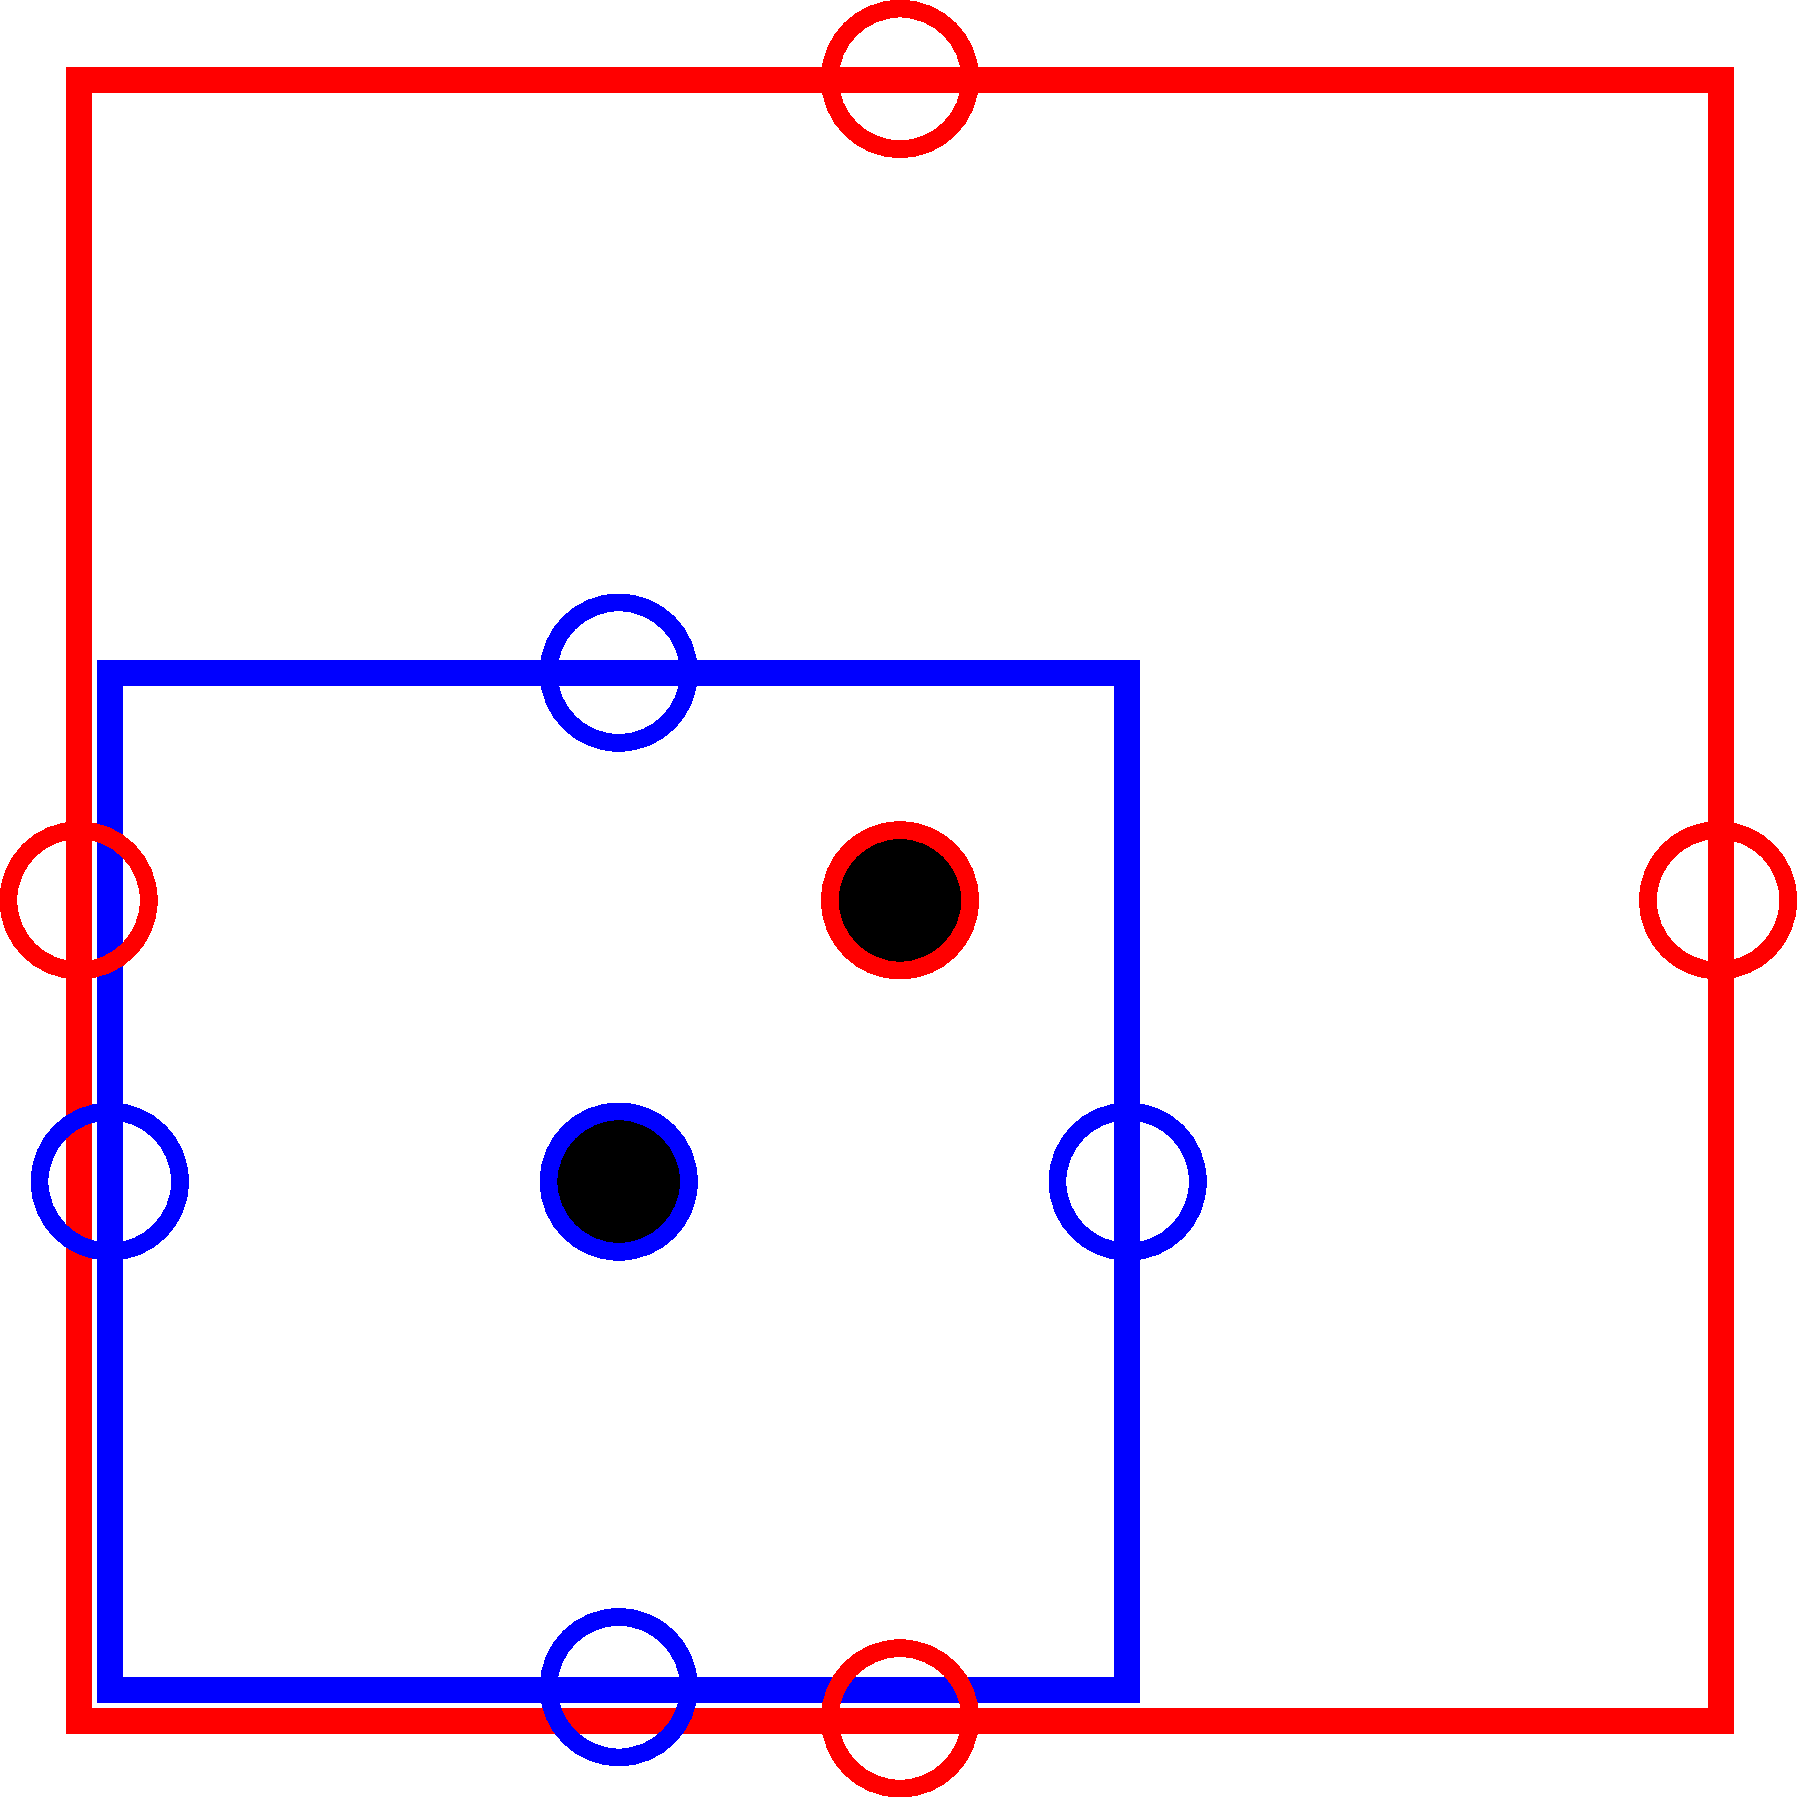
\includegraphics[width=0.6\textwidth]{drawings/audtestsetup}
    \caption{The setup for Room 1 and Room 2 (illustration of \Cref{fig:audtest}). Room 1 is marked as the inner (blue) square and is $5 \times 5$ meters. Room 2 is marked as the outer (red) square and is $8 \times 8$ meters. The rings shows the position of the beacons. The filled circles shows where the the phone is placed to obtain the position (only for the non-moving tests).}
    \label{fig:audtestsetup}
\end{figure}

\FloatBarrier
\subsection{Room 2}

\subsection{Room 3}

\subsection{Room 4}

\subsection{Conclusion}


We setup a [SIZE OF ROOM] room, with [NUMBER OF BEACONS]. 
The room is illustrated by \Cref{fig:precisiontest}. 
In \Cref{fig:precisiontest} you can also see small spots. 
These spots is the known locations where we are going to perform the precision tests. 
We randomly walk between these spots [NUMBER OF TIMES] and find the mean error rate.
\begin{figure}[!htb]
    \centering
    \todo[author=Thalley]{Insert figure}
    \caption{Illustration of room used for indoor location precision test}
    \label{fig:precisiontest}
\end{figure}

The mean error rate that we found is [RESULT]. 

\subsection{Precision of Indoor Location Conclusion}
From the results, we can conclude that... \todo[author=Thalley]{Write conclusion of precision test based on results}


\section{Overall System Correctness}\label{sec:systemcorrectness}
This test is designed to test the system as a whole. 
We want to test how many times the system:
\begin{enumerate}
    \item Sends the right action to the right device
    \item Sends the wrong action to the right device
    \item Sends the right action to the wrong device
    \item Sends the wrong action to the wrong device
\end{enumerate}
Thus this test is meant to total correctness of our system. 

We have the following setup, also illustrated in \Cref{fig:totalcorrectness}:
[SETUP: Which devices, where they are, where we stand, etc.]
\begin{figure}[!htb]
    \centering
    \todo[author=Thalley]{Insert figure}
    \caption{Illustration of our setup for the total correctness test}
    \label{fig:totalcorrectness}
\end{figure}

We send a total of [NUMBER OF GESTURES]. 
\Cref{table:correctnessresults} shows the results of this test.

\begin{table}
    \centering
    \begin{tabular}{l|cc}
                     & Right action & Wrong Action \\ \hline
        Right Device &      x       &     z        \\
        Wrong Device &      y       &     w        \\
    \end{tabular} 
    
    \todo[author=Thalley]{Insert results}
    \caption{Table showing the correctness of our system}
    \label{table:correctnessresults}
\end{table}

\subsection{Overall System Correctness Conclusion}
From the results, we can conclude that... \todo[author=Thalley]{Write conclusion of precision test based on results}
